Midblock crossings are crosswalks that are located on streets in places other than intersections.  They are a safer alternative to pedestrians jaywalking at unmarked points.  Most crosswalks are located at intersections, where traffic lights allow for vehicles to be controlled in order for pedestrians to safely cross the street.  In dense, urban locations with short blocks, this works well.  However, in areas with long stretches of road between intersections, it is not always convenient to have to cross at an intersection.  Many pedestrians will jaywalk across a street at the location where they need to cross it, not necessarily at an intersection.  This can present a hazard to both pedestrians and vehicles, as they could cross the street at any point, and approaching vehicles may not be able to see them.  One study shows that midblock jaywalking was responsible for 26.5\% of all pedestrian accidents \cite{mid1}.

With long blocks, long signals, wide intersections, and high vehicle speeds, crossing at intersections isn’t always easy.  It becomes important to identify points at which it is practical and safe to cross roads.  Without them, pedestrians make their own decisions to cross at random points, creating risk for both themselves and drivers.  By increasing the number of midblock crossings, we hope to decrease the occurrence of jaywalking while improving pedestrian mobility.

\begin{figure}[!htbp]
\centering
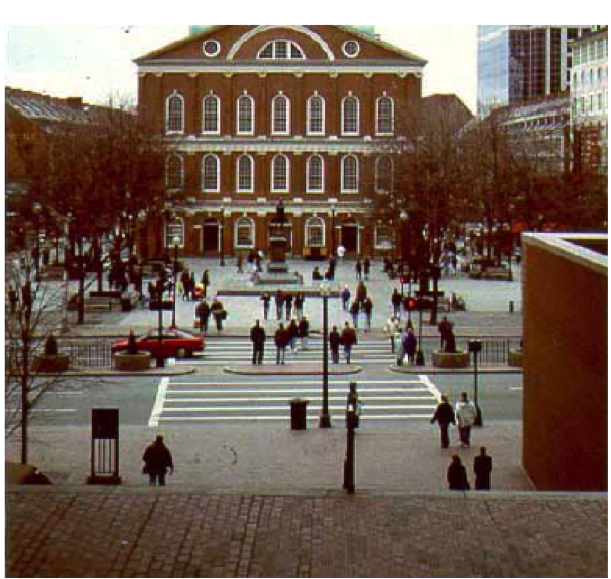
\includegraphics[width=0.5\textwidth]{midblock}
\caption[Midblock Crossing]{Midblock crossings safely connect public places between intersections.}\label{fig:midblock}
\end{figure}

\subsubsection{Medians}
Medians, also called refuge islands, are often necessary for high volume and high speed roads.  Without them, crosswalks are simply too long to cross.  They provide a convenient resting area halfway through a crosswalk where pedestrians can safely wait until the other lanes of traffic are safe to cross.  It can be difficult to find a suitable gap in traffic for multiple lanes, with traffic heading in both directions.  A median can cut the number of lanes in half by creating two separate crossing journeys, each with traffic in only one direction \cite{mid2}. 

For low volume and low speed roads, medians often are not necessary.  Gaps in traffic are easier to navigate, and the walking distance across the crosswalk is shorter.  For roads with traffic above 30 mph and high traffic volume, midblock crossings should utilize signals and other control devices \cite{mid2}.

\begin{figure}[!htbp]
\centering
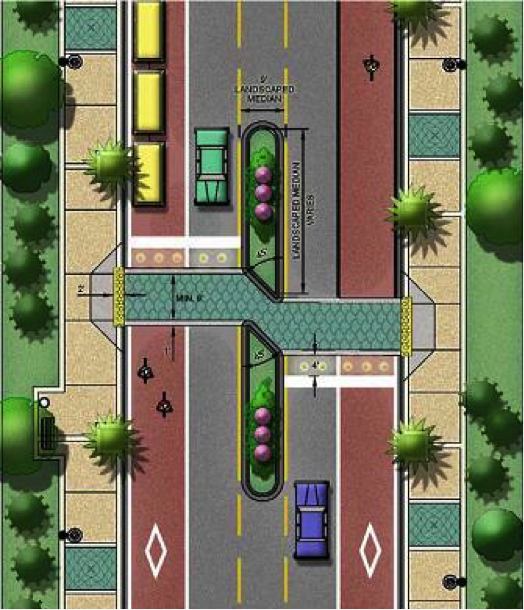
\includegraphics[width=0.5\textwidth]{median}
\caption[Median]{Medians divide long crosswalks into two shorter ones.}\label{fig:median}
\end{figure}

\subsubsection{Signals}
Signals are often necessary for multiple lane roads with high speeds, like those found in Los Angeles.   With multiple lane roads come a host of traffic conditions, such as vehicles changing lanes and speed.  These conditions can make it more challenging for pedestrians to identify gaps, as well as for vehicles to identify pedestrians.  With high speeds, traffic signals might be necessary for vehicles to have a sufficient stopping distance before a crosswalk.  Large signs, flashing lights, bulb outs and flashing signs have all been shown to work well at midblock crossings \cite{mid3}.  Midblock crossings are not always expected, so motorists might not be looking out for them.

Signals and signage can include:\begin{itemize}
	\item Pavement markings 
	\item New signage 
	\item Painted/textured surfaces 
	\item Flashing lights 
\end{itemize}

\begin{figure}[!htbp]
\centering
        \begin{subfigure}[t]{0.45\textwidth}
                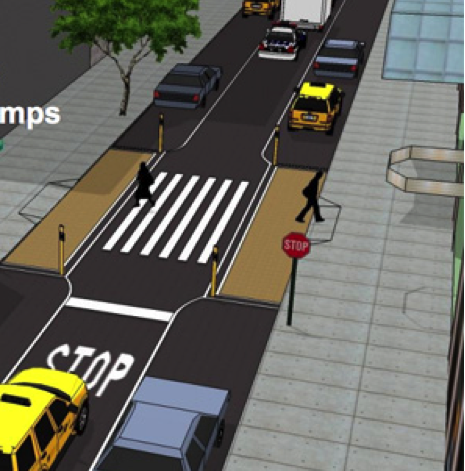
\includegraphics[width=\textwidth]{signage1}
                \caption{Stop signs and curb extensions}
                \label{fig:midsignage1}
        \end{subfigure}
        \begin{subfigure}[t]{0.45\textwidth}
                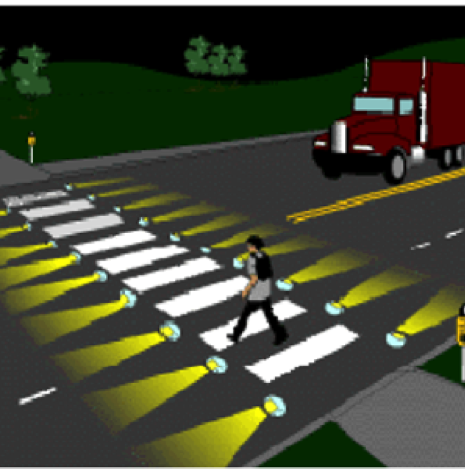
\includegraphics[width=\textwidth]{signage2}
                \caption{Flashing lights}
                \label{fig:midsignage2}
        \end{subfigure}
\caption[Midblock Crossing Design Tools]{Designing midblock crossings with these tools in mind increase pedestrian safety\cite{mid4}}
\end{figure}


\subsubsection{Staggering}

Staggered crosswalks (Z-crossings) are a special type of crossing that contain a median that offsets a set of crosswalks on either side of the median.  Since the overall crossing path is no longer a straight line, this forces pedestrians to turn and view oncoming traffic upon reaching the median before crossing the rest of the street \cite{mid2}.  This encourages pedestrians to look for oncoming traffic.

\begin{figure}
\centering
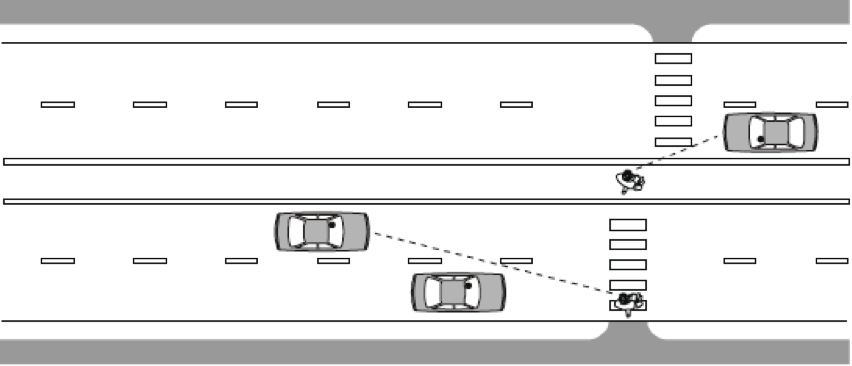
\includegraphics[width=0.7\textwidth]{stagger}
\caption[Staggered Crossing]{Staggered midblock crossings increase visibility of oncoming vehicles to pedestrians at the median\cite{mid3}.}
\end{figure}

\clearpage

\subsubsection{Estimated Costs}
% Booktabs require to add \usepackage{booktabs} to your document preamble
\begin{table}[h]
\centering
\begin{tabular}{@{}lr@{}}
\toprule
Design                                                                         & \multicolumn{1}{l}{Cost} \\ \midrule
Crosswalk (walk countdown) signal                                              & \$5,000                  \\
Curb extensions                                                                & $5,000 - $25,000         \\
Basic crosswalks with signs and markings                                       & $500 - $1,500            \\
Enhanced crosswalk with special stencils, raised platforms, or special signage & \$5,000                  \\
Raised crosswalks:                                                             & $2,000 – $15,000         \\
Refuge island (median)                                                         & $10,000 – $40,000        \\
In pavement illumination                                                       & $25,000 – $40,000        \\
Pedestrian only traffic signal                                                 & $40,000 - $75,000        \\
Midblock flashing crosswalk                                                    & \$40,000                \\
\bottomrule
\end{tabular}
\caption{Costs of midblock crossing design elements}
\end{table}

